% Figure 8: editable three-panel LaTeX layout matching Figure 4.
% \figeightpanelwidth is the final size; no outer scaling is applied.
\begin{figure}[!ht]
    \centering
    \begingroup
    \newlength{\figeightpanelwidth}
    \newlength{\figeightlegendunit}
    \setlength{\figeightpanelwidth}{1.55in}
    \setlength{\figeightlegendunit}{\dimexpr\figeightpanelwidth*10/52\relax}

    \definecolor{figeightTemp0}{RGB}{70,94,207}
    \definecolor{figeightTemp1}{RGB}{103,136,238}
    \definecolor{figeightTemp2}{RGB}{138,173,253}
    \definecolor{figeightTemp3}{RGB}{173,201,253}
    \definecolor{figeightTemp4}{RGB}{205,217,237}
    \definecolor{figeightTemp5}{RGB}{232,214,205}
    \definecolor{figeightTemp6}{RGB}{246,191,166}
    \definecolor{figeightTemp7}{RGB}{244,157,126}
    \definecolor{figeightTemp8}{RGB}{229,112,88}
    \definecolor{figeightTemp9}{RGB}{201,57,54}

    \newcommand{\figeightlegendbar}{%
        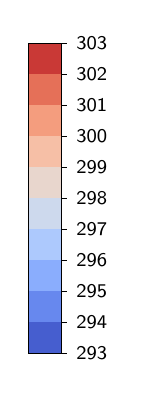
\begin{tikzpicture}[baseline=0pt,x=1cm,y=\figeightlegendunit]
            \fill[figeightTemp0] (0,0.00) rectangle (0.42,0.52);
            \fill[figeightTemp1] (0,0.52) rectangle (0.42,1.04);
            \fill[figeightTemp2] (0,1.04) rectangle (0.42,1.56);
            \fill[figeightTemp3] (0,1.56) rectangle (0.42,2.08);
            \fill[figeightTemp4] (0,2.08) rectangle (0.42,2.60);
            \fill[figeightTemp5] (0,2.60) rectangle (0.42,3.12);
            \fill[figeightTemp6] (0,3.12) rectangle (0.42,3.64);
            \fill[figeightTemp7] (0,3.64) rectangle (0.42,4.16);
            \fill[figeightTemp8] (0,4.16) rectangle (0.42,4.68);
            \fill[figeightTemp9] (0,4.68) rectangle (0.42,5.20);
            \draw[line width=0.35pt] (0,0) rectangle (0.42,5.20);
            \foreach \y/\ticklabel in {
                0.00/293,0.52/294,1.04/295,1.56/296,2.08/297,
                2.60/298,3.12/299,3.64/300,4.16/301,4.68/302,5.20/303}
                {\draw[line width=0.3pt] (0.42,\y) -- (0.49,\y)
                 node[anchor=west,font=\sffamily\fontsize{7.5}{8}\selectfont]
                 {\ticklabel};}
        \end{tikzpicture}%
    }

    \newcommand{\figeightpanellabel}[2]{%
        {\sffamily\bfseries\fontsize{8.5}{9.5}\selectfont
         (#1) $h_c/l_c=#2$}%
    }

    \begin{tabular}[c]{@{}l@{\hspace{0.10in}}c@{\hspace{0.05in}}c@{\hspace{0.05in}}c@{}}
        {\sffamily\bfseries\fontsize{8.5}{9.5}\selectfont Temperature} & & & \\[-1pt]
        \figeightlegendbar &
        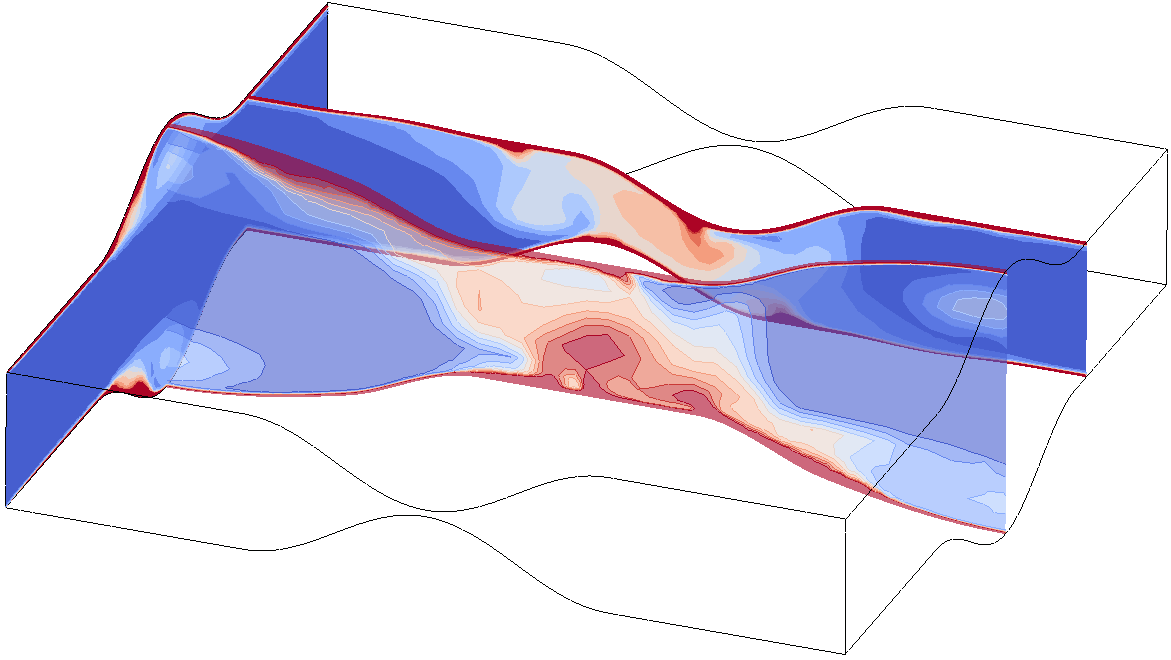
\includegraphics[width=\figeightpanelwidth]{image_2/Figure11/CH_2mm_Temp.png} &
        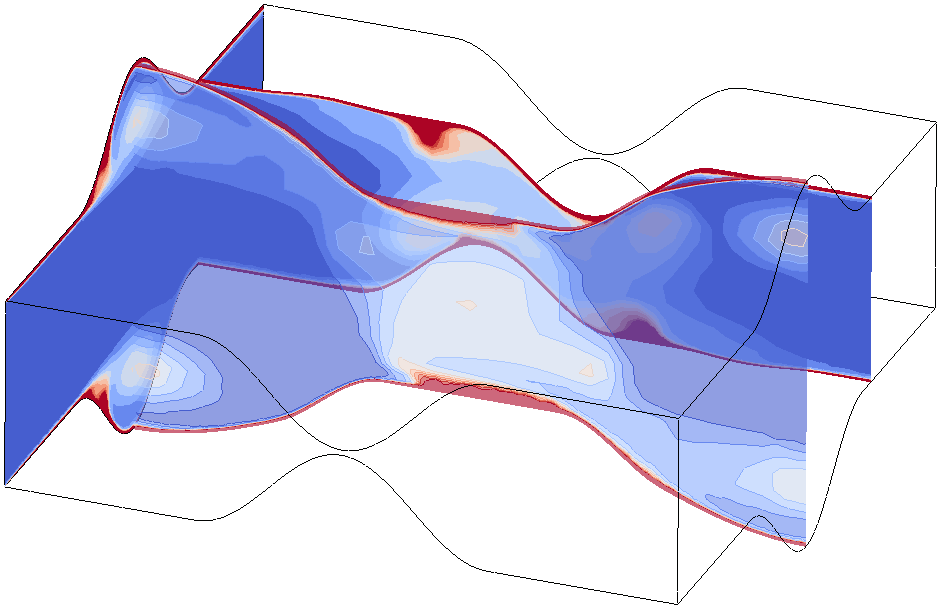
\includegraphics[width=\figeightpanelwidth]{image_2/Figure11/CH_3.5mm_Temp.png} &
        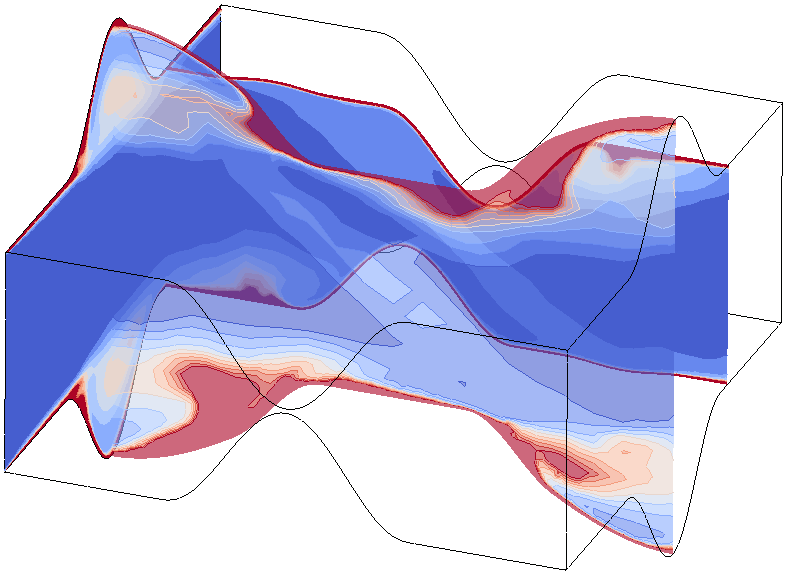
\includegraphics[width=\figeightpanelwidth]{image_2/Figure11/CH_5mm_Temp.png} \\[-1pt]
        {\sffamily\fontsize{7.5}{8.5}\selectfont $[\mathrm{K}]$} &
        \figeightpanellabel{a}{0.08} &
        \figeightpanellabel{b}{0.14} &
        \figeightpanellabel{c}{0.20}
    \end{tabular}
    \endgroup
    \caption{Temperature distribution of CPHE at representative normalized capsule heights ($h_c/l_c=0.08$, $0.14$, and $0.20$).}
    \label{figure8}
\end{figure}
